% Il faut commencer par la, c'est le plus simple: priorités
% statiques, préemption, RR, RM, EDF, Background, Serveur
% scrutation, Serveur différé, Serveur sporadique
\part{Ordonnancement}

\tikzstyle{cgreen}  = [fill=green!20!white,  draw=green!50!black,  line width=1pt, rounded corners=1pt]
\tikzstyle{cred}    = [fill=red!20!white,    draw=red!50!black,    line width=1pt, rounded corners=1pt]
\tikzstyle{cblue}   = [fill=blue!20!white,   draw=blue!50!black,   line width=1pt, rounded corners=1pt]
\tikzstyle{cpurple} = [fill=purple!20!white, draw=purple!50!black, line width=1pt, rounded corners=1pt]
\tikzstyle{corange} = [fill=orange!20!white, draw=orange!50!black, line width=1pt, rounded corners=1pt]
\tikzstyle{ccyan}   = [fill=cyan!20!white,   draw=cyan!50!black,   line width=1pt, rounded corners=1pt]
\tikzstyle{cbrown}  = [fill=brown!20!white,  draw=brown!50!black,  line width=1pt, rounded corners=1pt]
\tikzstyle{cyellow} = [fill=yellow!20!white, draw=yellow!50!black, line width=1pt, rounded corners=1pt]

\def\lo#1{ -- ++(#1,0) }
\def\hi#1{ |- ++(#1,1) -- ++(0,-1) }
\def\hop#1#2{\lo{#1}\hi{#2}}

\def\timeline#1#2#3{
  \draw[xstep=1,ystep=1.5,gray,very thin] (0,0) grid (#1.5,#2);
  \draw[->, line width=1pt] (0,#2) -- (#1.5,#2) coordinate (x axis);
  \draw[line width=1pt] (0,#2) -- (0,0) coordinate (x axis);
  \foreach \x in {0,1,...,#1}
    \draw (\x.5,#2) node[anchor=north] {\tiny\x};
  \foreach \y/\ytext in {#3}
    \draw (0,\y) node[anchor=east] {\ytext};
}

\section{Quelques notions théoriques}

\subsection{Modèle de tâches}

\begin{frame}{Modèle de tâches}
  Paramètres définissant une tâche $i$:
  \begin{itemize}
    \item Date d'arrivée de la tâche dans le système : $S_i$
    \item Première date d'activation : $R_i$
    \item Période d'activation : $P_i$
    \item Délai critique (délai maximum acceptable pour son exécution)
      : $D_i$
    \item Capacité (Temps CPU nécessaire à l'éxecution de la tâche) :
      $C_i$
    \item Date de réveil sur une période $k$ : $r_{ik}$
    \item Echéance sur une période $k$ : $d_{ik} = r_{ik} + D_i$
  \end{itemize}
  \note{Ajouter le schéma de Touchard}
\end{frame}

\begin{frame}{Modèle de tâches}
  Par conséquent: 
  \begin{itemize} 
  \item Tâche périodique définie par : $(S_i, R_i, P_i ,D_i, C_i)$
  \item Tâche apériodique définie par : $(S_i, R_i, 0, D_i, C_i)$
  \end{itemize} 
  Très souvent:
  \begin{itemize}
    \item Les tâches sont connues début de l'ordonnacement : $S_i = 0$
    \item Les tâches périodique sont actives dès le début de
      l'ordonnancement : $R_i = 0$
    \item L'échéance des  tâches périodique est leur période  : $D_i =
      P_i$
  \end{itemize}
\end{frame}

\begin{frame}{Modèle de tâches}
  Paramètres statiques:
  \begin{itemize} 
  \item Facteur d'utilisation du processeur: $U_i =  C_i /P_i$
  \item Facteur de charge du processeur : $CH_i = C_i / D_i $ ($CH_i =
    U_i$ si échéance sur périodes)
  \item Laxité de la tâche (retard maximum acceptable pour l'exécution
    de la tâche) : $L_i = D_i - C_i$
  \end{itemize} 
  Paramètres dynamiques (dépendant de l'ordonnancement):
  \begin{itemize} 
  \item Date du début de l'exécution d'une période $k$ : $s_{ik}$
  \item Date de la fin de l'exécution d'une période $k$ :$e_{ik}$
  \item Temps de réponse de la tâche $TR_{ik} = e_{ik} - r_{ik}$ (Nous
    verrons comment le calculer)
    % = C_i + \sum_{prio(j) > prio(i)} \left\lceil\frac{TR_i}{P_j}\right\rceil C_j$
  \item Durée d'exécution résiduelle à la date $t$ : $C_i(t)$ ($0 \leq
    C_i(t) \leq C_i$)
  \item Délai  critique résiduel à la  date $t$ :  $D_i(t) = d_{ik}-t$
    ($0 \leq D_i(t) \leq D_i$)
  \item Charge résiduelle à la date $t$ :
    $CH_i(t) = C_i(t) / D_i(t)$  ($0 \leq CH_i(t) \leq CH_i$)
  \item Laxité  résiduelle à la  date $t$ :
    $L_i(t) = D_i(t) - C_i(t)$  ($0  \leq L_i(t) \leq  L_i$)
  \item  Laxité conditionnelle  à la  date $t$  (somme sur  les tâches
    déclenchées à la  date $t$ et qui sont devant $i$  du point de vue
    de  l'ordonnancement)  :  $LC_i(t)  =  D_i(t)  -  \sum_{prio(j)  >
      prio(i)} C_j(t)$ ($0 \leq LC_i(t) \leq L_i$)
  \end{itemize} 
\end{frame}

\note{Peut-etre ajouter slide 5 de Touchar}
\note{J'ai placé le slide 7 avant le slide 6 de touchard}

\begin{frame}{Paramètres du système}
  \begin{itemize} 
  \item  Configuration  :  ensemble   des  tâches  mises  en  jeu  par
    l'application
  \item Taux d'utilisation du processeur : $U = \sum_i U_i$
  \item Taux de charge du processeur : $CH = \sum_i CH_i$
  \item Intervalle d'étude :  intervalle de temps minimum pour prouver
    l'ordonnançabilité  d'une  configuration. Dans  le  cas de  tâches
    périodiques: $ppcm_i(P_i)$
  \item Laxité du  processeur : intervalle de temps  pendant lequel le
    processeur peut rester inactif  tout en respectant les échéances :
    $ LP(t) = \min(LC_i(t))$
  \end{itemize} 
\end{frame} 

\begin{frame}{Etats des tâches}
  \begin{center}
    \begin{tikzpicture}[scale=2]
      \node (Wa)  at (2,1) {Waiting};
      \node (In)  at (0,0) {};
      \node (Re)  at (1,0) {Ready};
      \node (Ru)  at (2,0) {Running};
      \node (Out) at (3,0) {};
      \node (Int) at (2,-1) {Interrupt};
      \draw[->] (Re)  -- (Ru);
      \draw[->] (Ru)  -- (Wa);
      \draw[->] (Ru)  -- (Int);
      \draw[->] (Int) -- (Ru);
      \draw[->] (Wa)  -- (Re);
      \draw[->] (Ru)  -- (Out);
      \draw[->] (In)  -- (Re);
    \end{tikzpicture}
  \end{center}
\end{frame} 

\subsection{Théroème de l'instant critique}

\begin{frame}{Théorème de l'instant critique}
  Si toutes les  tâches arrivent initialement dans le  système en même
  temps et  si elles respectent  leur première échéance,  alors toutes
  les  échéances  seront  respectées  par  la  suite,  quel  que  soit
  l'instant d'arrivée des tâches.

  \begin{itemize}
  \item  C'est une condition  nécessaire et  suffisante si  toutes les
    tâches du système sont initialement prêtes au même instant.
  \item Dans le cas contraire, c'est une condition suffisante
  \end{itemize}

  Si $D_i = P_i$, le test de terminaison est :
  $$\forall i, 1 \leq i \leq n \;\;\;\min_{0 \leq t \leq D_i}
  \sum_{j=1}^i\frac{C_j}{t}
  \left\lfloor\frac{t}{P_j}\right\rfloor \leq 1$$
\end{frame}

\subsection{Temps de réponse}

\begin{frame}{Temps de réponse}
  Délai entre l'activation d'une tâche et sa terminaison. 

  $$TR_i = C_i + \sum_{prio(j) > prio(i)} \left\lceil\frac{TR_i}{T_j}\right\rceil C_j$$

\end{frame}

\begin{frame}{Calcul du temps de réponse}
  Technique de calcul : on évalue de façon itérative
  $$w_i^{n+1}=C_i+\sum_{prio(j) > prio(i)} \left\lceil\frac{w_i^n}{P_j}\right\rceil C_j$$

  \begin{itemize}
    \item On démarre avec $w_i^0 = C_i$
    \item Echec si $w_i^n > P_i$
    \item Réussite si $w_i^{n+1} = w_i^n$
  \end{itemize}
\end{frame} 

\begin{frame}{Calcul du temps de réponse}
  \textbf{Exemple :}
    \begin{center}
      \begin{tabular}{ccccc}
        \hline
        Tâche & Arrivée & Période & Capacité & Echéance \\
        \hline
        A & 0 &  7 & 3 & Fin de période\\
        B & 0 & 12 & 2 & Fin de période\\
        C & 0 & 20 & 5 & Fin de période\\
        \hline
      \end{tabular}
    \end{center}
    \begin{itemize} 
      \item $w_1^0 = C_1 = 3$
      \item $w_2^0 = C_2 = 2$
      \item $w_2^1 = 2 + 3 \left\lceil\frac{2}{7}\right\rceil = 5$
      \item $w_2^2 = 2 + 3 \left\lceil\frac{5}{7}\right\rceil = 5$
      \item $w_3^0 = C_3 = 5$
      \item $w_3^1 = 5 + 3 \left\lceil\frac{5}{7}\right\rceil + 2 \left\lceil\frac{5}{12}\right\rceil = 10$
      \item $w_3^2 = 5 + 3 \left\lceil\frac{10}{7}\right\rceil + 2 \left\lceil\frac{10}{12}\right\rceil = 13$
      \item $w_3^3 = 5 + 3 \left\lceil\frac{13}{7}\right\rceil + 2 \left\lceil\frac{13}{12}\right\rceil = 15$
      \item $w_3^4 = 5 + 3 \left\lceil\frac{15}{7}\right\rceil + 2 \left\lceil\frac{15}{12}\right\rceil = 18$
      \item $w_3^5 = 5 + 3 \left\lceil\frac{18}{7}\right\rceil + 2 \left\lceil\frac{18}{12}\right\rceil = 18$
      \end{itemize} 
\end{frame}

\section{Algorithmes à priorité statique}

\begin{frame}{Typologie des algorithmes}
  On distingue diverse typologie d'algorithmes:
  \begin{itemize}
  \item  \emph{on  line}  ou   \emph{off  line}:  Choix  dynamique  ou
    prédéfini à la conception
  \item  à priorité \emph{statique}  ou \emph{dynamique}:  La priorité
    d'une  tâche est-elle  fixe  ou une  variable dépendante  d'autres
    paramètres 
  \item \emph{préemptif} ou  \emph{non préemptif}: Une tâche peut-elle
    perdre le  processeur (au profit d'une tâche  plus prioritaire) ou
    non
  % \item stratégie du meilleur effort ou inclémence
  %   \begin{itemize}
  %   \item  en  TR mou,  meilleur  effort =  faire  au  mieux avec  les
  %     processeurs disponibles
  %   \item  en  TR  dur,   obligation  des  respecter  les  contraintes
  %     temporelles : inclémence aux fautes temporelles
  %   \end{itemize}
  %\item centralisé ou réparti
  \end{itemize}
\end{frame}

\begin{frame}{Round-Robin}
TODO
\end{frame} 

\subsection{Rate Monotonique (RM)}

\begin{frame}{Algorithme}
  Ordonnancement à priorité statique où les priorité sont inversement
  proportionnelles aux périodes des tâches. 

  Fonctionne  en version préemptive.  La version  non-préemptive n'est
  pas garantie.

  Liu et Layland ont démontré qu'un système est ordonnançable si le
  taux d'occupation du processeur $U$ vérifie la condition suffisante
  (non nécessaire) suivante :
  $$U = \sum_i^n \frac{C_i}{T_i} \leq n \left(2^{\frac{1}{n}}-1\right)$$

  \begin{center}
    \begin{tabular}{cc}
      \hline
      $n$ & limite d'occupation \\
      \hline
      1 & 100.0\% \\
      2 & 82.8\% \\
      3 & 78.0\% \\
      4 & 75.7\% \\
      5 & 74.3\% \\
      10 & 71.9\% \\
      $\infty$ & 69.3\%\\
      \hline
    \end{tabular}
  \end{center}
\end{frame}

\begin{frame}{Exemple 1}
  \begin{center}
    \begin{tabular}{ccccc}
      \hline
      Tâche & Arrivée & Période & Capacité & Echéance \\
      \hline
      A & 0 & 20 & 8 & Fin de période\\
      B & 0 & 10 & 1 & Fin de période\\
      C & 0 &  4 & 1 & Fin de période\\
      \hline
    \end{tabular}
  \end{center}
  Charge du CPU:
  $$\frac{8}{40} + \frac{1}{10} + \frac{1}{4} = 0.75$$
\end{frame} 

\begin{frame}{Exemple 1}
  Mode préemptif ($ppcm(4, 10, 20) = 20$):\\ 
  % CBAACAAACABACAAACXXX
  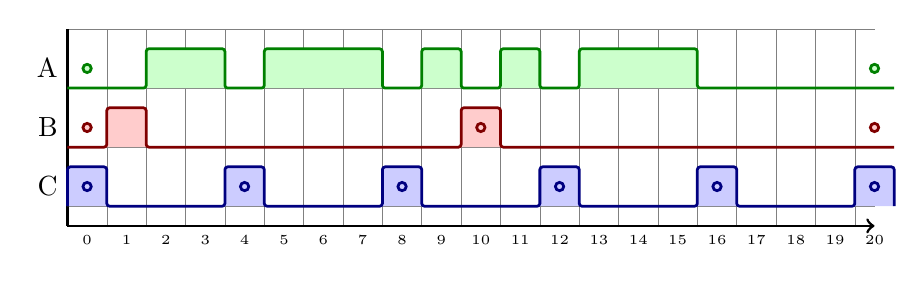
\begin{tikzpicture}[scale=0.5]
    \timeline{20}{-5}{-1.0/A, -2.5/B, -4.0/C}
    \fill[cgreen] (0,-1.5) \lo 1 \lo 1 \hi 2 \lo 1 \hi 3 \lo 1 \hi 1 \lo 1 \hi 1 \lo 1 \hi 3 \lo 1 \lo 3 \lo 1;
    \fill[cred]   (0,-3.0) \lo 1 \hi 1 \lo 2 \lo 1 \lo 3 \lo 1 \lo 1 \hi 1 \lo 1 \lo 1 \lo 3 \lo 1 \lo 3 \lo 1;
    \fill[cblue]  (0,-4.5) \hi 1 \lo 1 \lo 2 \hi 1 \lo 3 \hi 1 \lo 1 \lo 1 \lo 1 \hi 1 \lo 3 \hi 1 \lo 3 \hi 1;
    \foreach \i in {0, 20}
      \draw[cgreen] (\i + 0.5, -1) circle (3pt);
    \foreach \i in {0, 10, 20}
      \draw[cred]   (\i + 0.5, -2.5) circle (3pt);
    \foreach \i in {0, 4, ..., 20}
      \draw[cblue]  (\i + 0.5, -4) circle (3pt);
    \end{tikzpicture}
    \\
    Mode non-préemptif :\\ 
    % CBAAAAAAAAAACCCBXCXXX
    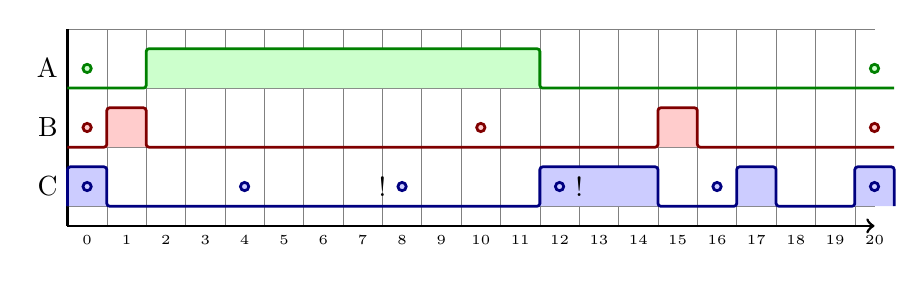
\begin{tikzpicture}[scale=0.5]
      \timeline{20}{-5}{-1.0/A, -2.5/B, -4.0/C}
      \fill[cgreen] (0,-1.5) \lo 1 \lo 1 \hi{10} \lo 3 \lo 1 \lo 1 \lo 1 \lo 2 \lo 1;
      \fill[cred]   (0,-3.0) \lo 1 \hi 1 \lo{10} \lo 3 \hi 1 \lo 1 \lo 1 \lo 2 \lo 1;
      \fill[cblue]  (0,-4.5) \hi 1 \lo 1 \lo{10} \hi 3 \lo 1 \lo 1 \hi 1 \lo 2 \hi 1;
      \foreach \i in {0, 20}
        \draw[cgreen] (\i + 0.5, -1) circle (3pt);
      \foreach \i in {0, 10, 20}
        \draw[cred]   (\i + 0.5, -2.5) circle (3pt);
      \foreach \i in {0, 4, ..., 20}
        \draw[cblue]  (\i + 0.5, -4) circle (3pt);
      \draw[cred] (8, -4) node {!};
      \draw[cred] (13, -4) node {!};
    \end{tikzpicture}
\end{frame}

\begin{frame}{Exemple 2}
    \begin{center}
      \begin{tabular}{ccccc}
        \hline
        Tâche & Arrivée & Période & Capacité & Echéance \\
        \hline
        A & 0 & 16 & 8 & Fin de période\\
        B & 0 &  8 & 2 & Fin de période\\
        C & 0 &  4 & 1 & Fin de période\\
        \hline
      \end{tabular}
    \end{center}
    $$\frac{8}{16} + \frac{2}{8} + \frac{1}{4} = 1$$
\end{frame}

\subsection{Deadline Monotonic}
\note{ajouter un exemple montrant la différence entre les deux}

\begin{frame}{Deadline Monotonic (DM)} 
  \begin{itemize}
  \item Algorithme à priorité statique
\item Généralisation de Rate Monotonic aux tâches à échéance sur requête
  \item Basé sur le délai critique :
    \begin{itemize}
    \item La tâche de plus petit délai critique est la plus prioritaire
    \end{itemize}
\item Test d'acceptabilité:
  $$U = \sum_i^n \frac{C_i}{D_i} \leq n \left(2^{\frac{1}{n}}-1\right)$$
  \item Equivalent à Rate Monotonic  dans le cas des tâches à échéance
    sur requête, meilleur dans les autres cas
  \end{itemize}
\end{frame}

\begin{frame}{Exemple}
  \begin{center}
    \begin{tabular}{ccccc}
      \hline
      Tâche & Arrivée & Période & Capacité & Echéance \\
      \hline
      A & 0 & 20 & 3 & 7\\
      B & 0 &  5 & 2 & 4\\
      C & 0 & 10 & 2 & 9\\
      \hline
    \end{tabular}
  \end{center}
\end{frame} 

\begin{frame}{Exemple}
  Par RM:
  $$\frac{3}{20} + \frac{2}{5} + \frac{2}{10} = 0.75$$
  % BBCCABBAAXBBCC
  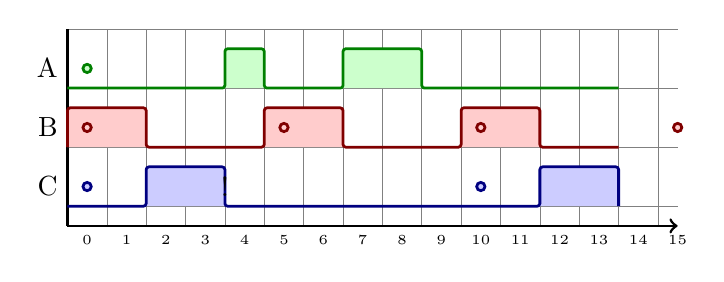
\begin{tikzpicture}[scale=0.5]
    \timeline{15}{-5}{-1.0/A, -2.5/B, -4.0/C}
    \fill[cgreen] (0,-1.5) \lo 2 \lo 2 \hi 1 \lo 2 \hi 2 \lo 1 \lo 2 \lo 2;
    \fill[cred]   (0,-3.0) \hi 2 \lo 2 \lo 1 \hi 2 \lo 2 \lo 1 \hi 2 \lo 2;
    \fill[cblue]  (0,-4.5) \lo 2 \hi 2 \lo 1 \lo 2 \lo 2 \lo 1 \lo 2 \hi 2;
    \foreach \i in {0}
      \draw[cgreen] (\i + 0.5, -1)   circle (3pt);
    \foreach \i in {0, 5, 10, 15}
      \draw[cred]   (\i + 0.5, -2.5) circle (3pt);
    \foreach \i in {0, 10}
      \draw[cblue]  (\i + 0.5, -4)   circle (3pt);
    \draw[cred] (4, -4) node {!};
  \end{tikzpicture}

  Par DM:
  $$\frac{3}{7} + \frac{2}{4} + \frac{2}{9} = 1.15$$
  % BBAAABBCCXBBCC
  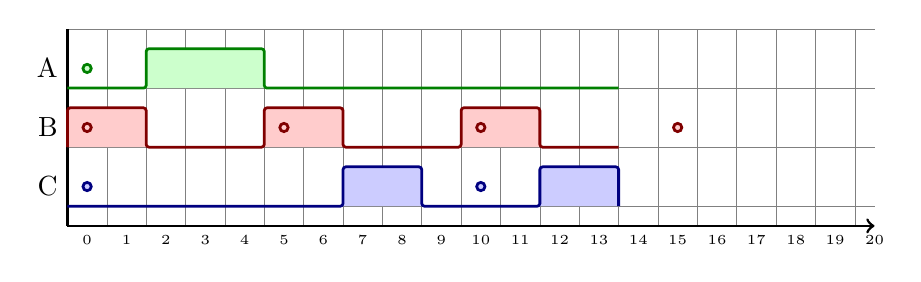
\begin{tikzpicture}[scale=0.5]
    \timeline{20}{-5}{-1.0/A, -2.5/B, -4.0/C}
    \fill[cgreen] (0,-1.5) \lo 2 \hi 3 \lo 2 \lo 2 \lo 1 \lo 2 \lo 2;
    \fill[cred]   (0,-3.0) \hi 2 \lo 3 \hi 2 \lo 2 \lo 1 \hi 2 \lo 2;
    \fill[cblue]  (0,-4.5) \lo 2 \lo 3 \lo 2 \hi 2 \lo 1 \lo 2 \hi 2;
    \foreach \i in {0}
      \draw[cgreen] (\i + 0.5, -1) circle (3pt);
    \foreach \i in {0, 5, 10, 15}
      \draw[cred]   (\i + 0.5, -2.5) circle (3pt);
    \foreach \i in {0, 10}
      \draw[cblue]  (\i + 0.5, -4) circle (3pt);
  \end{tikzpicture}
\end{frame} 

\section{Algorithmes à priorité dynamique}

\subsection{Earliest Deadline First (EDF)}

\begin{frame}{Algorithme EDF}
  \begin{itemize}
  \item Algorithme à priorité dynamique
  \item Basé sur l'échéance :
    \begin{itemize}
    \item A chaque instant (i.e à chaque réveil de tâche), la priorité
      maximale  est donnée  à la  tâche  dont l'échéance  est la  plus
      proche
    \end{itemize}
  \item Test d'acceptabilité:
    \begin{itemize}
    \item Condition nécessaire:
      $$U = \sum_i^n \frac{C_i}{P_i} \leq 1$$
    \item Condition suffisante:
      $$U = \sum_i^n \frac{C_i}{D_i} \leq 1$$
    \item  Dans le  cas  de tâche  à  échéance sur  requête, les  deux
      conditions sont égales
    \end{itemize}
  \end{itemize}
\end{frame}

\begin{frame}{Exemple}
  \begin{center}
    \begin{tabular}{ccccc}
      \hline
      Tâche & Arrivée & Période & Capacité & Echéance \\
      \hline
      A & 0 & 20 & 3 & 7\\
      B & 0 &  5 & 2 & 4\\
      C & 0 & 10 & 2 & 8\\
      \hline
    \end{tabular}
  \end{center}
    $$\frac{3}{20} + \frac{2}{5} + \frac{2}{10} = 0.75 \leq 1$$
    $$\frac{3}{7} + \frac{2}{4} + \frac{2}{9} = 1.15 > 1$$
    % BBAAACCBBXBBCCXBBXXX
    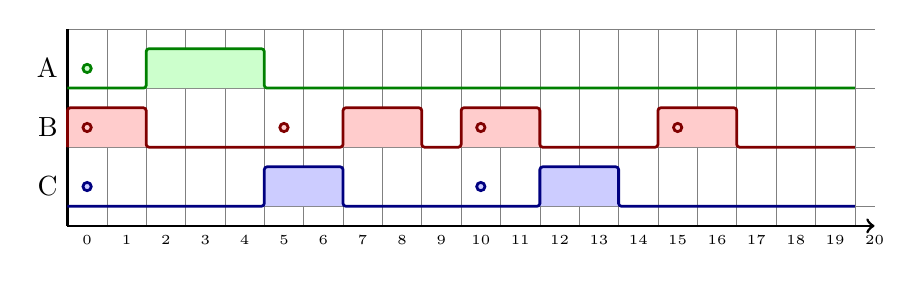
\begin{tikzpicture}[scale=0.5]
      \timeline{20}{-5}{-1.0/A, -2.5/B, -4.0/C}
      \fill[cgreen] (0,-1.5) \lo 2 \hi 3 \lo 2 \lo 2 \lo 1 \lo 2 \lo 2 \lo 1 \lo 2 \lo 3;
      \fill[cred]   (0,-3.0) \hi 2 \lo 3 \lo 2 \hi 2 \lo 1 \hi 2 \lo 2 \lo 1 \hi 2 \lo 3;
      \fill[cblue]  (0,-4.5) \lo 2 \lo 3 \hi 2 \lo 2 \lo 1 \lo 2 \hi 2 \lo 1 \lo 2 \lo 3;
      \foreach \i in {0}
        \draw[cgreen] (\i + 0.5, -1.0) circle (3pt);
      \foreach \i in {0, 5, 10, 15}
        \draw[cred]   (\i + 0.5, -2.5) circle (3pt);
      \foreach \i in {0, 10}
        \draw[cblue]  (\i + 0.5, -4.0) circle (3pt);
    \end{tikzpicture}
\end{frame} 
  
\subsection{LST}

\begin{frame}{Least Slack Time (LST)} 
  \begin{itemize}
  \item Algorithme à priorité dynamique
  \item Aussi appelé \emph{Least Laxity First (LLF)}
  \item   Amélioration   de  EDF.   Mêmes   propriétée,  mais   permet
    d'ordonnancer des problèmes non-ordonnancable par EDF.
  \item Basé sur la laxité résiduelle: 
    \begin{itemize}
    \item La  priorité maximale est  donnée à la  tâche qui a  la plus
      petite laxité résiduelle: $L(t) = D(t) - C(t)$
    \end{itemize}
  \item Equivalent à  EDF si on ne calcule la  laxité qu'au réveil des
    tâches
  \item Optimum à trouver entre  la granularité du calcul et le nombre
    de changements de  contexte provoqués 
    \note{Effectivement,  dans   un  EDF  ou  RM,   on  recalcule  que
      lorsqu'une tache revient dans l'ordonanceur (= lorsqu'elle passe
      de SLEEP  à RUN =sur evenement  = rare).  Ici il  faut choisr un
      quantum pour le  calcul de la laxité.  Néanmoins,  c'est deja ce
      qu'on fait des que l'on souhaite faire du round robin.}
  \end{itemize}
\end{frame}

\begin{frame}{Exemple}
  \begin{center}
    \begin{tabular}{ccccc}
      \hline
      Tâche & Arrivée & Période & Capacité & Echéance \\
      \hline
      A & 0 & 20 & 4 & 12\\
      B & 0 &  5 & 1 & 4\\
      C & 0 & 10 & 6 & 8\\
      \hline
    \end{tabular}
  \end{center}
  Avec un quantum de temps de 1:
  \note{Meme résultat que pour EDF. Trouver un autre exemple. Il faut une tache avec une forte capacité et une forte échéance.}
 %      3    B    2    B    3  
 % LST: CCBCCCCBAAAABCCCCCCXX
 % EDF: BCCCCCCBAAAABCCCCCCXX
 %                  
\end{frame} 

\section{Serveurs de tâches apériodiques}


\begin{frame}{Introduction} 
  \begin{itemize}
  \item Tâches prises en compte dans une configuration comprenant déjà
    des tâches périodiques
  \item A priori, on ne  connaît pas l'instant d'arrivée de la requête
    de réveil de la tâche apériodique
  \item Contraintes temporelles strictes ou relatives 
  \item Buts à atteindre : 
    \begin{itemize}
    \item Maintenir les garanties du temps réelles sur les tâches déjà
      présentes dans l'ordonnanceur
    \item Si contraintes relatives : minimiser le temps de réponse
    \item  Si contraintes  strictes :  maximiser le  nombre  de tâches
      acceptées en respectant leurs contraintes
    \end{itemize}
  \end{itemize}
\end{frame}

\subsection{Execution en arrière-plan}

\begin{frame}{Traitement en arrière-plan} 
  \begin{itemize}
  \item Aussi appellé \emph{backgound} ou sur \emph{temps creux}
  \item tâches apériodiques ordonnancées quand le processeur est oisif 
    \begin{itemize}
    \item les tâches périodiques restent les plus prioritaires 
    \end{itemize}
  \item ordonnancement relatif des tâches apériodiques en mode FIFO 
  \item traitement le plus simple, mais le moins performant 
  \item Pas de  marge de manoeuvre pour améliorer  le temps de réponse
    des  tâches apériodique.  Potentiellement, les  tâches apériodique
    peuvent avoir des temps de réponse long.
  \end{itemize}
\end{frame}

\begin{frame}{Traitement en arrière-plan} 
  Avec ordonnancement RM des tâches périodiques:
  \begin{center}
    \begin{tabular}{ccccc}
      \hline
      Tâche & Arrivée & Période & Capacité & Echéance \\
      \hline
      A & 0 &  5 & 2 & Fin de période\\
      B & 0 & 10 & 2 & Fin de période\\
      1 & 0 &  3 & 2 & Aucune\\
      2 & 0 & 10 & 1 & Aucune\\
      3 & 0 & 11 & 2 & Aucune\\
      \hline
    \end{tabular}
  \end{center}
  % AABB1AA1X2AABB1AA33
  % Temps de réponses:
  % 1: 2: 3:
\end{frame} 

\subsection{Traitement par serveur}

\begin{frame}{Traitement par serveur} 
  \begin{itemize}
  \item un  serveur est une  tâche périodique créée  spécialement pour
    prendre en compte les tâches apériodiques
  \item serveur caractérisé par :
    \begin{itemize}
    \item sa période 
    \item son temps d'exécution : capacité du serveur  
    \item serveur  généralement ordonnancé suivant  le même algorithme
      que les autres tâches périodiques
    \item une fois actif, le serveur sert les tâches apériodiques dans
      la limite de sa capacité.
    \item l'ordre de traitement  des tâches apériodiques ne dépend pas
      de l'algorithme général
    \end{itemize}
  \item Il est  possible de le combiner le  traitement avec un serveur
    avec   un   traitement   en   background   (Temps   de   réponse+,
    prédictabilité-)
  \end{itemize}
\end{frame}

\subsection{Serveur par scrutation}

\begin{frame}{Serveur par scrutation}
  \begin{itemize}
  \item Aussi appellé \emph{polling}
  \item A chaque activation,  traitement des tâches en suspens jusqu'à
    épuisement  de la capacité  ou jusqu'à  ce qu'il  n'y ait  plus de
    tâches en attente
  \item Si aucune tâche n'est  en attente (à l'activation ou parce que
    la  dernière  tâche  a  été  traitée)  ,  le  serveur  se  suspend
    immédiatement et perd sa capacité qui peut être réutilisée par les
    tâches périodiques
  \item Quand une instance (un événement) de tâche apériodique arrive,
    elle attend jusqu’à ce que la capacité du serveur soit disponible.
  \item  Il est  possible de  rendre la  main au  CPU si  aucune tache
    apériodique  n'est  en  attente  (TR  des  taches  periodiques  +,
    prédictabilité -)
  \item  Dans  le  cas  ou  le  serveur à  la  plus  petite  priorité,
    l'algorithme équivaut à peu près au traitement en background
  \end{itemize}
\end{frame} 

\begin{frame}{Exemple}
  A vide, avec ordonnancement RM des tâches périodiques:
  \begin{center}
    \begin{tabular}{ccccc}
      \hline
      Tâche & Arrivée & Période & Capacité & Echéance \\
      \hline
      A & 0 & 20 & 3 & Fin de période\\
      B & 0 & 10 & 2 & Fin de période\\
      S & 0 &  5 & 2 & Fin de période\\
      \hline
    \end{tabular}
  \end{center}
  % SSBBASSAAXSSBBXSS
\end{frame} 

\begin{frame}{Exemple}
  Idem avec les 3 tâches apériodiques:
  \begin{center}
    \begin{tabular}{ccccc}
      \hline
      Tâche & Arrivée & Période & Capacité & Echéance \\
      \hline
      A & 0 & 20 & 3 & Fin de période\\
      B & 0 & 10 & 2 & Fin de période\\
      S & 0 &  5 & 2 & Fin de période\\
      1 & 0 &  3 & 2 & Aucune\\
      2 & 0 & 10 & 1 & Aucune\\
      3 & 0 & 11 & 2 & Aucune\\
      \hline
    \end{tabular}
  \end{center}
  % SSBBA11AAX23BBX3S
\end{frame} 

\begin{frame}{Exemple}
  Idem, en libérant le temps CPU inutilisé par le serveur:
  \begin{center}
    \begin{tabular}{ccccc}
      \hline
      Tâche & Arrivée & Période & Capacité & Echéance \\
      \hline
      A & 0 & 20 & 3 & Fin de période\\
      B & 0 & 10 & 2 & Fin de période\\
      S & 0 &  5 & 2 & Fin de période\\
      1 & 0 &  3 & 2 & Aucune\\
      2 & 0 & 10 & 1 & Aucune\\
      3 & 0 & 11 & 2 & Aucune\\
      \hline
    \end{tabular}
  \end{center}
  % BBAAA11XXX23BBX3XXXX
\end{frame} 

\subsection{Serveur différé}

\begin{frame}{Limitation} 
  Limitations du serveur par scrutation 
  \begin{itemize}
  \item perte de la capacité si aucune tâche apériodique en attente
  \item si occurrence d'une tâche apériodique alors que le serveur est
    suspendu, il faut attendre la requête suivante
  \end{itemize}
\end{frame} 

\begin{frame}{Serveur différé}
  Aussi appellé serveur ajournable
  La fausse bonne idée
  Provoque des erreur d'ordonnancement
\end{frame}

\begin{frame}{Exemple}
 % Reprendre le cas du dos à dos
\end{frame} 

\subsection{Serveur sporadique}

\begin{frame}{Serveur sporadique}
  \begin{itemize}
  \item  améliore le  temps de  réponse des  tâches  apériodiques sans
    diminuer  le  taux d'utilisation  du  processeur  pour les  tâches
    périodiques
  \item Très utilisé pour les  IHM car permet une meilleure expérience
    utilisateur
  \item comme le serveur différé mais 
    \begin{itemize}
    \item  ne retrouve  pas  sa capacité  à  période fixe,  mais à  un
      instant de réinitialisation égal  à la date courante additionnée
      de la période de réinitialisation
      \item la capacité retrouvée est égale à la capacité consommée 
      \end{itemize}
    \end{itemize}
\end{frame} 

\begin{frame}{Exemple}
  Avec ordonnancement RM:
  \begin{center}
    \begin{tabular}{ccccc}
      \hline
      Tâche & Arrivée & Période & Capacité & Echéance \\
      \hline
      A & 0 & 20 & 3 & Fin de période\\
      B & 0 & 10 & 2 & Fin de période\\
      S & 0 &  5 & 2 & Fin de période\\
      1 & 0 &  3 & 2 & Aucune\\
      2 & 0 & 10 & 1 & Aucune\\
      3 & 0 & 11 & 2 & Aucune\\
      \hline
    \end{tabular}
  \end{center}
  % BBAA11AXXX23BBX3
  % Changer d'exemple, il ne fait aucune différence avec le serveur par scrutation
  % Hint: reprendre le cas d'execution dos à dos
\end{frame} 


